\documentclass[11pt]{article}

\usepackage[czech]{babel}
\usepackage{a4wide}
\usepackage[utf8]{inputenc}
\usepackage[T1]{fontenc}
\usepackage{fancyhdr}
\usepackage{amssymb}
\usepackage{amsthm}
\usepackage{amsmath}
\usepackage{mathtools}
\usepackage{mleftright}
\usepackage{subcaption}
\usepackage{gensymb}
\usepackage{parskip}
\usepackage{titlesec}
\usepackage{subfiles}
\usepackage[bottom]{footmisc}  % forcing footnotes to be at the very bottom

\usepackage{geometry}
\geometry{
    a4paper,
    total={170mm,257mm},
    right=20mm,
    left=20mm,
    top=30mm,
    bottom=20mm,
}


% ---------------------------------------- KÓD ----------------------------------------
\usepackage[outputdir=Build]{minted}
\setminted{
frame=lines,
framesep=2mm,
linenos,
autogobble
}


% ---------------------------------------- BIBLIOGRAFIE ----------------------------------------
\usepackage[backend=biber, style=numeric]{biblatex}
\addbibresource{main.bib}


% ---------------------------------------- JEDNOTKY ----------------------------------------
\usepackage{siunitx}
\sisetup{per-mode = symbol}


% ---------------------------------------- FLOATY ----------------------------------------
\usepackage{float}
\floatplacement{figure}{H}


% ---------------------------------------- PŘÍKLADY ----------------------------------------
% https://tex.stackexchange.com/questions/164113/the-exercise-package-in-list-form
\usepackage{scrextend}
\usepackage[load-headings]{exsheets}
\DeclareInstance{exsheets-heading}{mylist}{default}{
  runin = true ,
  attach = {
    main[l,vc]number[l,vc](-2em,0pt) ;
    main[l,vc]title[l,vc](-5.5em,0pt)
  }
}

\DeclareRobustCommand*\questionstar{\texorpdfstring{\bonusquestionsign}{* }}
\DeclareRobustCommand*\questionstartwo{\texorpdfstring{\bonusquestionsigntwo}{* }}
\DeclareRobustCommand*\bonusquestionsign{\llap{$\bigstar$\space}}
\DeclareRobustCommand*\bonusquestionsigntwo{\llap{$\bigstar\bigstar$\space}}

\NewQuSolPair
	{question*}[name=\questionstar Příklad]
	{solution*}[name=\questionstar Řešení]

\NewQuSolPair
	{question**}[name=\questionstartwo Příklad]
	{solution**}[name=\questionstartwo Řešení]

\DeclareTranslation{Czech}{exsheets-exercise-name}{Příklad}
\DeclareTranslation{Czech}{exsheets-solution-name}{Řešení}

\SetupExSheets{
  headings = mylist , % use the new headings instance
  headings-format = \it ,
  counter-format = se.qu ,
  counter-within = section ,
	question/pre-hook = \addmargin[5.5em]{0em} ,
	solution/pre-hook = \addmargin[5.5em]{0em} ,
	question/post-hook = \endaddmargin ,
	solution/post-hook = \endaddmargin
}

% https://tex.stackexchange.com/questions/263467/exsheets-how-to-get-a-counter-reference-combining-section-and-question-numbers
\renewcommand\thequestion{\thesection.\arabic{question}}


% ---------------------------------------- LINKY ----------------------------------------
\usepackage{hyperref}
\urlstyle{same}
\hypersetup{
    colorlinks=true,
    urlcolor=blue,
    linkcolor=black,%TOC
}


% ---------------------------------------- NADPISY ----------------------------------------
\titleformat{\section} {\normalfont\fontsize{16}{15}\bfseries}{\thesection}{1em}{}
\titleformat{\subsection} {\normalfont\fontsize{14}{15}\bfseries}{\thesubsection}{1em}{}
\titleformat{\subsubsection} {\normalfont\fontsize{12}{15}\bfseries}{\thesubsubsection}{1em}{}

\usepackage{tcolorbox}
\tcbset{on line,
        boxsep=4pt, left=0pt,right=0pt,top=0pt,bottom=0pt,
        colframe=white
        }


% ---------------------------------------- HLAVIČKA ----------------------------------------
\pagestyle{fancy}
\fancyhf{}
% Now set the headers
\fancyhead[LE,RO]{\footnotesize\thepage}
\fancyhead[LO,RE]{\footnotesize\leftmark}
\fancyfoot{}
\fancyfoot[R]{\thepage}


% ---------------------------------------- BARVY ----------------------------------------
\definecolor{ceruleanblue}{rgb}{0.16, 0.32, 0.75}
\definecolor{motorlight}{rgb}{0.85, 0.80, 0.70}
\definecolor{motordark}{rgb}{0.64, 0.51, 0.25}
\definecolor{wait}{rgb}{0.64, 0.25, 0.25}


% ---------------------------------------- DEFINICE BLOKŮ ----------------------------------------
\newcommand{\block}{$\vcenter{\hbox{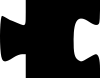
\includegraphics[height=0.8em]{../Images/blocky-logo.png}}}$}
\newcommand{\centerimage}[2]{$\vcenter{\hbox{\includegraphics[height=#1]{#2}}}$}


\newcommand{\blockMotorStart}{\item[\block] \centerimage{2em}{../Images/blocks/motor-start.png} -- \parbox{0.545\textwidth}{zapne daný motor dopředu (\textit{forward}) nebo dozadu (\textit{reverse}) na danou rychlost (\textit{velocity}) v procentech.}}
\newcommand{\blockMotorStop}{\item[\block] \centerimage{1.6em}{../Images/blocks/motor-stop.png} -- vypne daný motor.}
\newcommand{\blockMotorDistance}{\item[\block] \centerimage{2em}{../Images/blocks/motor-distance-start.png} -- \parbox{0.525\textwidth}{zapne motor, dokud se neotočí o daný počet stupňů (\textit{degrees}) nebo otáček (\textit{revolutions}). Je neblokující -- zapne motor a jde na další block.}}
\newcommand{\blockMotorVelocity}{\item[\block] \centerimage{2em}{../Images/blocks/motor-velocity.png} -- nastaví rychlost motoru, ale nezapne ho!}

\newcommand{\blockMotorDoneImage}{\centerimage{1.6em}{../Images/blocks/motor-done.png} }
\newcommand{\blockMotorDone}{\item[\block] \blockMotorDoneImage -- podmínka která říká, zda daný motor skončil.}

\newcommand{\blockLoop}{\item[\block] \centerimage{4em}{../Images/blocks/loop.png} -- opakuje bloky uvnitř několikrát.}
\newcommand{\blockLoopForever}{\item[\block] \centerimage{4em}{../Images/blocks/loop-forever.png} -- opakuje bloky uvnitř donekonečna.}
\newcommand{\blockLoopWhile}{\item[\block] \centerimage{4em}{../Images/blocks/loop-while.png} -- \parbox{0.725\textwidth}{opakuje bloky uvnitř, dokud (\textit{while}) nebo než (\textit{until}) platí podmínka.}}

\newcommand{\blockWaitImage}{\centerimage{2em}{../Images/blocks/wait.png} }
\newcommand{\blockWait}{\item[\block] \blockWaitImage -- čeká daný čas.}
\newcommand{\blockWaitUntil}{\item[\block] \centerimage{1.6em}{../Images/blocks/wait-until.png} -- čeká, než (\textit{until}) platí podmínka.}
\newcommand{\blockStartImage}{\centerimage{1.6em}{../Images/blocks/start.png} }
\newcommand{\blockStart}{\item[\block] \blockStartImage -- startovní blok pro každý Blocky program.}

\newcommand{\blockFunctionDefinition}{\item[\block] \centerimage{4em}{../Images/blocks/function-definition.png} -- definování funkce; jméno lze upravit kliknutím.}
\newcommand{\blockFunctionCall}{\item[\block] \centerimage{2em}{../Images/blocks/function-call.png} -- volání funkce TODO lepší vysvětlení?.}

\newcommand{\blockBumperPressed}{\item[\block] \centerimage{1.6em}{../Images/blocks/bumper-pressed.png} -- podmínka, která říká, zda je daný senzor stisknutý.}

\newcommand{\blockVariableCreate}{\item[\block] \centerimage{1.6em}{../Images/blocks/variable-create.png} -- vytvoří novou proměnnou.}
\newcommand{\blockVariableChange}{\item[\block] \centerimage{1.6em}{../Images/blocks/variable-change.png} -- změní danou proměnnou o dané číslo.}
\newcommand{\blockVariableGet}{\item[\block] \centerimage{1.6em}{../Images/blocks/variable-get.png} -- hodnota dané proměnné.}
\newcommand{\blockVariableSet}{\item[\block] \centerimage{1.6em}{../Images/blocks/variable-set.png} -- nastaví hodnotu dané proměnné.}


% ---------------------------------------- SDÍLENÉ PŘÍKAZY ----------------------------------------
\newcommand{\errata}{%
	\subsection{Chyby, překlepy, doplňky}
	Pokud někde odhalíte chybu/překlep, nebo máte pocit, že by něco šlo napsat lépe, tak mě buďto kontaktuje na adrese \href{mailto:tomas@slama.dev}{tomas@slama.dev}, nebo vytvořte issue/pull request na stránce \url{https://github.com/xiaoxiae/uvod-do-programovani-vex-v5}.
}
